\documentclass[border=15pt]{standalone}
\usepackage{tikz,amsmath}
\usetikzlibrary{arrows.meta}

% ========== 配色方案 ==========
\definecolor{inFill}{RGB}{183,224,177}       % 输入特征图绿色
\definecolor{inLine}{RGB}{32,102,32}
\definecolor{hidFill}{RGB}{199,203,243}     % 卷积核紫色
\definecolor{hidLine}{RGB}{52,58,143}
\definecolor{outFill}{RGB}{243,199,199}     % 输出特征图红色
\definecolor{outLine}{RGB}{143,52,52}

\begin{document}
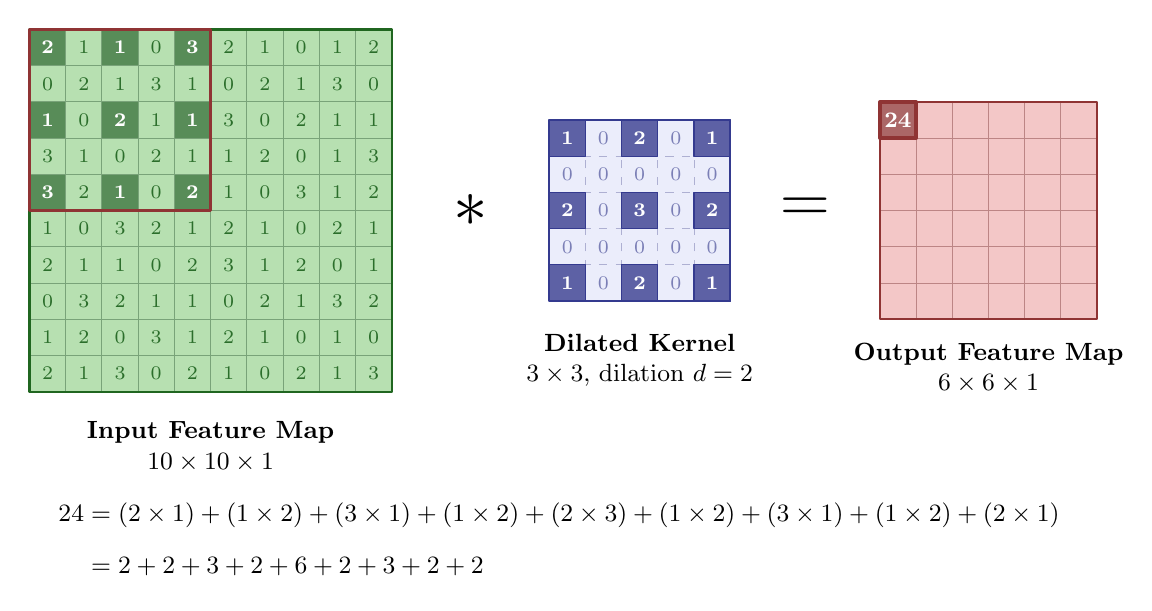
\begin{tikzpicture}[
    font=\small, line join=round,
    every node/.style={inner sep=0pt, outer sep=0pt, align=center}
  ]

  % 1. 左侧：输入特征图 (10x10，单元格 0.46cm)
  \fill[inFill] (0, -2.3) rectangle ++(4.6, 4.6);

  % 9 个深绿高亮采样单元格 (d=2 采样点)
  \foreach \r in {0,2,4} {
    \foreach \c in {0,2,4} {
      \fill[inLine!75] ({0 + \c*0.46}, {2.3 - (\r+1)*0.46}) rectangle ++(0.46, 0.46);
      \draw[inLine, line width=.4pt] ({0 + \c*0.46}, {2.3 - (\r+1)*0.46}) rectangle ++(0.46, 0.46);
    }
  }

  % 网格线
  \draw[step=0.46, inLine!60, line width=.35pt] (0, -2.3) grid ++(4.6, 4.6);

  % 逐行填入数字宏 (规避 TikZ 嵌套列表展开 bug)
  \newcommand{\fillinrow}[2]{%
    \foreach \val [count=\c from 0] in {#2} {
      \pgfmathtruncatemacro{\isSampled}{((\c==0 || \c==2 || \c==4) && (#1==0 || #1==2 || #1==4)) ? 1 : 0}
      \ifnum\isSampled=1
        \node[font=\fontsize{7.5}{8.5}\selectfont\bfseries, text=white]
          at ({0 + (\c+0.5)*0.46}, {2.3 - (#1+0.5)*0.46}) {\val};
      \else
        \node[font=\fontsize{7}{8}\selectfont, text=inLine!95]
          at ({0 + (\c+0.5)*0.46}, {2.3 - (#1+0.5)*0.46}) {\val};
      \fi
    }%
  }

  \fillinrow{0}{2, 1, 1, 0, 3, 2, 1, 0, 1, 2}
  \fillinrow{1}{0, 2, 1, 3, 1, 0, 2, 1, 3, 0}
  \fillinrow{2}{1, 0, 2, 1, 1, 3, 0, 2, 1, 1}
  \fillinrow{3}{3, 1, 0, 2, 1, 1, 2, 0, 1, 3}
  \fillinrow{4}{3, 2, 1, 0, 2, 1, 0, 3, 1, 2}
  \fillinrow{5}{1, 0, 3, 2, 1, 2, 1, 0, 2, 1}
  \fillinrow{6}{2, 1, 1, 0, 2, 3, 1, 2, 0, 1}
  \fillinrow{7}{0, 3, 2, 1, 1, 0, 2, 1, 3, 2}
  \fillinrow{8}{1, 2, 0, 3, 1, 2, 1, 0, 1, 0}
  \fillinrow{9}{2, 1, 3, 0, 2, 1, 0, 2, 1, 3}

  % 红色框覆盖 5x5 感受野跨度
  \draw[inLine, thick] (0, -2.3) rectangle ++(4.6, 4.6);
  \draw[outLine, line width=1.3pt] (0, 0) rectangle (2.3, 2.3);

  % 底部标题
  \node[align=center] at (2.3, -3.0) {\textbf{Input Feature Map}\\$10\times 10\times 1$};

  % 卷积乘号 *
  \node[font=\Huge] at (5.6, 0) {$\ast$};

  % 2. 中间：有效核 5x5 (dilation=2)
  \fill[hidFill!35] (6.6, -1.15) rectangle ++(2.3, 2.3);
  \draw[step=0.46, hidLine!40, dashed, line width=.35pt, shift={(6.6, -1.15)}] (0,0) grid (2.3, 2.3);

  % 卷积核逐行填入数值宏
  \newcommand{\fillkrow}[2]{%
    \foreach \kval [count=\c from 0] in {#2} {
      \pgfmathtruncatemacro{\isTap}{((\c==0 || \c==2 || \c==4) && (#1==0 || #1==2 || #1==4)) ? 1 : 0}
      \ifnum\isTap=1
        \fill[hidLine!80] ({6.6 + \c*0.46}, {1.15 - (#1+1)*0.46}) rectangle ++(0.46, 0.46);
        \draw[hidLine, line width=.4pt] ({6.6 + \c*0.46}, {1.15 - (#1+1)*0.46}) rectangle ++(0.46, 0.46);
        \node[font=\fontsize{7.5}{8.5}\selectfont\bfseries, text=white]
          at ({6.6 + (\c+0.5)*0.46}, {1.15 - (#1+0.5)*0.46}) {\kval};
      \else
        \node[font=\fontsize{7}{8}\selectfont, text=hidLine!65]
          at ({6.6 + (\c+0.5)*0.46}, {1.15 - (#1+0.5)*0.46}) {0};
      \fi
    }%
  }

  \fillkrow{0}{1, 0, 2, 0, 1}
  \fillkrow{1}{0, 0, 0, 0, 0}
  \fillkrow{2}{2, 0, 3, 0, 2}
  \fillkrow{3}{0, 0, 0, 0, 0}
  \fillkrow{4}{1, 0, 2, 0, 1}

  \draw[hidLine, thick] (6.6, -1.15) rectangle ++(2.3, 2.3);

  % 底部标题 (对齐基线至 Y = -3.0)
  \node[align=center] at (7.75, -1.9) {\textbf{Dilated Kernel}\\$3\times 3$, dilation $d=2$};

  % 等号 =
  \node[font=\Huge] at (9.85, 0) {$=$};

  % 3. 右侧：输出特征图 (6x6)
  \fill[outFill] (10.8, -1.38) rectangle ++(2.76, 2.76);
  \draw[step=0.46, outLine!60, line width=.35pt, shift={(10.8, -1.38)}] (0,0) grid (2.76, 2.76);

  % 左上角高亮并精确写入计算结果 24
  \fill[outLine!75] (10.8, 0.92) rectangle ++(0.46, 0.46);
  \draw[outLine, line width=1.3pt] (10.8, 0.92) rectangle ++(0.46, 0.46);
  \node[font=\fontsize{8.5}{9.5}\selectfont\bfseries, text=white]
    at ({10.8 + 0.5*0.46}, {1.38 - 0.5*0.46}) {24};

  \draw[outLine, thick] (10.8, -1.38) rectangle ++(2.76, 2.76);

  % 底部标题 (对齐基线至 Y = -3.0)
  \node[align=center] at (12.18, -2.0) {\textbf{Output Feature Map}\\$6\times 6\times 1$};

  % 4. 底部正中央公式：24 的详细点积计算过程
  \node at (6.78, -4.2) {
    $\begin{aligned}
      24 &= (2\times 1) + (1\times 2) + (3\times 1) + (1\times 2) + (2\times 3) + (1\times 2) + (3\times 1) + (1\times 2) + (2\times 1) \\[5pt]
         &= 2 + 2 + 3 + 2 + 6 + 2 + 3 + 2 + 2
    \end{aligned}$
  };

\end{tikzpicture}
\end{document}